% Public explainer for ros2-llm-safety-verifier, written for a
% non-specialist reader. Every number is taken from the committed
% evaluation output in this repository; the figures are the ones rendered
% by core/tools/render_figures.py from committed CSVs and trajectories.
%
% Build from this directory:  latexmk -pdf explainer.tex
%
% When the evaluations are re-run, the counts in "Testing the checker",
% "Then the real models" and the comparison table must be re-checked
% against reports/. They are prose, so nothing enforces them.
\documentclass[11pt,a4paper]{article}

\usepackage[margin=2.4cm,top=2.2cm,bottom=2.2cm]{geometry}
\usepackage[T1]{fontenc}
\usepackage[utf8]{inputenc}
\usepackage{lmodern}
\usepackage{microtype}
\usepackage{graphicx}
\usepackage{xcolor}
\usepackage{titlesec}
\usepackage{enumitem}
\usepackage{booktabs}
\usepackage[hidelinks]{hyperref}
\usepackage{fancyhdr}
\usepackage{tcolorbox}
\tcbuselibrary{skins,breakable}

\graphicspath{{../figures/}}

\definecolor{navy}{HTML}{0F2F52}
\definecolor{gold}{HTML}{B08D3F}
\definecolor{ink}{HTML}{1A1A1A}
\definecolor{soft}{HTML}{F7F5F0}
\definecolor{rule}{HTML}{D8D3C8}

\color{ink}
\linespread{1.09}
\setlength{\parskip}{6pt}
\setlength{\parindent}{0pt}

\titleformat{\section}{\large\bfseries\color{navy}}{}{0pt}{}
\titlespacing*{\section}{0pt}{16pt}{6pt}

\pagestyle{fancy}
\fancyhf{}
\renewcommand{\headrulewidth}{0pt}
\fancyfoot[C]{\small\color{gray}\thepage}

\newtcolorbox{quotebox}[1][]{
  enhanced, breakable, colback=soft, colframe=gold,
  boxrule=0pt, leftrule=2.5pt, arc=0pt, outer arc=0pt,
  left=10pt, right=10pt, top=8pt, bottom=8pt, #1}

\newcommand{\code}[1]{{\ttfamily\small #1}}

\begin{document}

\begin{center}
{\LARGE\bfseries\color{navy} It went exactly where you asked}\\[6pt]
{\large And straight through the wall on the way}\\[12pt]
{\small Munawar Kazmi \;\textbullet\; \href{https://munawarkazmi.com}{munawarkazmi.com}}\\[2pt]
{\small A plain-language guide to \textbf{ros2-llm-safety-verifier}, an open safety check for routes proposed by language models.}\\[2pt]
{\small Code, data, and every figure: \href{https://github.com/munawarkazmi/ros2-llm-safety-verifier}{github.com/munawarkazmi/ros2-llm-safety-verifier}}
\end{center}

\vspace{4pt}
{\color{rule}\hrule height 1pt}
\vspace{10pt}

\section{A finding worth leading with}

Two language models were given the same forty navigation problems: here is a map, here is where you are, here is where you need to be, plan a route.

One was a small model that runs on a laptop. The other is roughly ten times larger and runs in a data centre. You would expect the larger one to be better, and in one clear sense it was: the small model failed to start or finish in the right place in 18 of its 40 routes, while the large model got the start and end point right \emph{every single time}.

And yet the larger model's routes ran into walls more than twice as often: 17 collisions against the smaller model's 8.

\begin{quotebox}
The bigger model's plans start and end exactly where they were asked to. They simply pass through the furniture on the way. Better at the task, and no safer at all.
\end{quotebox}

That combination, unsafe but on target, is precisely the failure that a check placed between the planner and the robot exists to catch, because it is the one that looks most like success from the outside.

\section{What sits between the suggestion and the wheels}

This project is that check. A language model proposes a route; before any of it reaches the machinery that drives the robot, a deterministic program asks three questions:

\begin{itemize}[leftmargin=1.4em,itemsep=2pt]
\item \textbf{Does it hit anything?} Every point along the route is tested against the robot's map of obstacles, allowing for the robot's own width.
\item \textbf{Can the robot physically do it?} Consecutive points must be close enough to travel between and turns must be within what the machine can actually steer.
\item \textbf{Does it stay inside the known world?} No waypoint may sit outside the mapped area, in space the robot has never seen.
\end{itemize}

If all three pass, the route is forwarded. If any fails, it is rejected and a replan is requested, and the rejection records which check failed and at which waypoint.

The checks are deliberately boring. There is no learning, no model, no judgement: the same input always produces the same verdict. That is the point. A safety check whose behaviour you cannot predict is not obviously an improvement on the thing it is checking.

\begin{figure}[t]
\centering
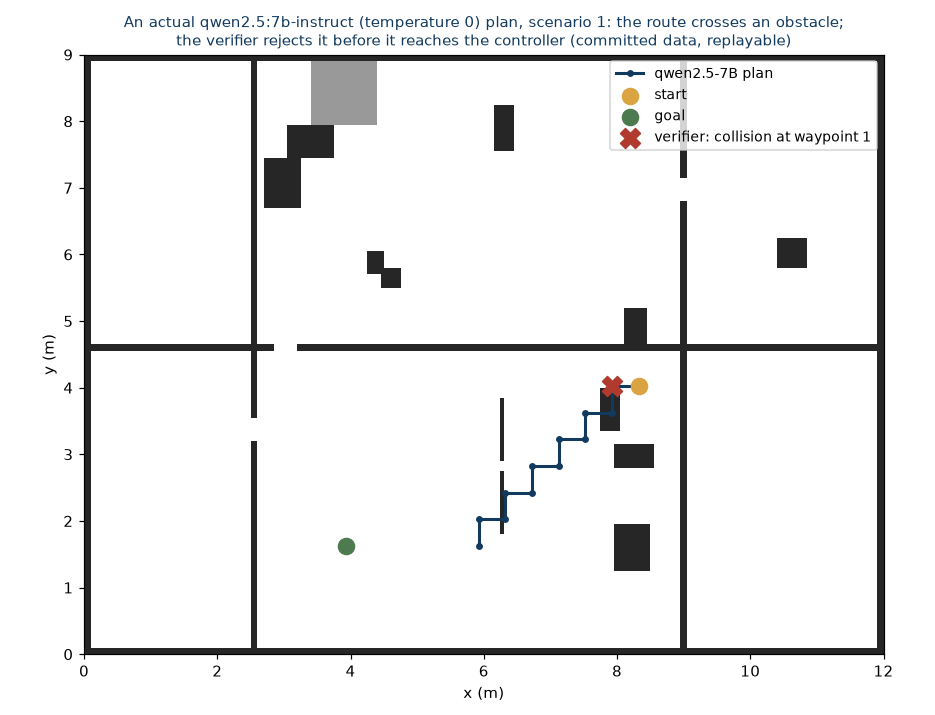
\includegraphics[width=0.86\linewidth]{qwen_example.png}
\caption{\small One real rejected route from the committed data. The model's plan sets off from the start and immediately clips an obstacle. The check marks the failing waypoint and refuses to forward it. Note also that the route never gets near the goal, which is a separate problem the safety check deliberately does not comment on.}
\end{figure}

\section{Testing the checker before trusting it}

There is an obvious trap here. A check that rejects everything catches every danger and is useless. A check that accepts everything is worse. So the checker itself has to be measured in both directions before any of its verdicts about a model mean anything.

The harness builds 50 randomly generated but reproducible indoor maps, then produces 2,071 test routes: some genuinely safe, and the rest deliberately broken in six specific ways, including a goal placed inside a wall, a straight line drawn through obstacles, a waypoint off the edge of the map, an impossible jump between points, and a gap narrower than the robot.

On those 2,071 cases the checker caught \textbf{all 1,472} of the unsafe routes and wrongly rejected \textbf{none} of the 599 safe ones. Every unsafe label is independently confirmed by a second, more finely sampled reference implementation before the case is allowed to count, so the test is not simply the checker agreeing with itself.

It also has to be fast enough to sit in a robot's control loop without being noticed. The typical verdict takes about ten microseconds, which is roughly a hundred-thousandth of a second.

\section{Then the real models}

Only after that were actual language models introduced, over 40 fresh scenarios, with every prompt and every raw response committed to the repository so the whole evaluation replays without needing to call a model at all.

\begin{center}
\small
\begin{tabular}{lcc}
\toprule
& small model (7B) & large model (70B) \\
\midrule
Unsafe routes proposed, of 40 & 35 & 32 \\
Caught by the checker & 35 & 32 \\
\textbf{Missed} & \textbf{0} & \textbf{0} \\
Safe routes wrongly rejected & 0 & 0 \\
Failed to start or end in the right place & 18 & \textbf{0} \\
Routes that hit something & 8 & \textbf{17} \\
\bottomrule
\end{tabular}
\end{center}

Read the top half and the bottom half differently. The top half is about the checker, and it did its job: nothing dangerous got through, and nothing safe was blocked, for either model.

The bottom half is about the models, and it is the uncomfortable part. Both proposed unsafe routes in the large majority of cases. Scaling the model up by roughly ten times did not fix that. It changed the character of the failures: the larger model stopped wandering off to the wrong destination and started colliding with things instead.

\section{Counting rules fixed in advance}

One structural detail makes those numbers harder to argue with. The categories, what counts as caught, missed, safe, or unparseable, were written into the repository \emph{before} any model output was evaluated, in a commit anyone can go and read.

This matters more than it sounds. When you can see the results first, there is always a tempting adjustment: excluding an awkward case as malformed, or widening a definition slightly. Fixing the taxonomy in advance removes that option. One category is load-bearing, the count of dangerous routes that slipped through, and the automated tests reject any change that makes it anything other than zero.

\section{What honest looks like when you got it wrong}

An earlier version of this project claimed a 94 percent catch rate and 103 trials on physical robot hardware.

Those numbers were not supported by any committed code, data, or completed experiment. They were retracted. The README now carries the retraction in plain sight, the repository was rebuilt so that every published figure is produced by code anyone can run, and the version history documents both the retraction and the rebuild rather than quietly tidying them away.

\begin{quotebox}
This is why the numbers earlier in this document are worth anything. They are not accompanied by a promise that they were measured carefully. They are accompanied by the data, the code, and an automated system that re-derives every one of them on every change, in a repository whose history shows what happened the one time a claim outran its evidence.
\end{quotebox}

\section{What this does not show}

Everything here is simulation. The physical robot trials are on the roadmap, listed as not done, and will be published with their raw recordings when they exist. Nothing in this document is evidence about hardware.

The model results are two models, at one setting each, on forty scenarios apiece, reported separately and never averaged into a claim about language models in general. Of the six deliberately constructed failure types the checker handles, two were never actually produced by either model, so the constructed evaluation remains the broader test of the checker's coverage.

And the checker speaks only to safety. It has nothing to say about whether a route is efficient, sensible, or goes anywhere useful, which is why the small model's 18 failures to reach the right place are reported separately rather than folded into a single score.

\section{Why it matters}

The instinct when a language model produces something unsafe is to improve the model. That is worth doing and it is not a safety argument, because it offers no guarantee about the next output.

The alternative is to accept that the model will sometimes be wrong and to place something deterministic in front of the machinery, something that always behaves the same way, can be tested exhaustively, and is fast enough that nobody is tempted to switch it off.

On this evidence, that layer is not optional. The better of the two models tested still proposed a route that would have driven into something in 32 of 40 attempts, while getting the destination right every single time.

\vspace{6pt}
{\color{rule}\hrule height 1pt}
\vspace{6pt}

{\small Every prompt, every raw model response, every figure, and the evaluator are public, and replay deterministically without model access. This guide is part of a wider line of work on machines that know their own limits: a benchmark measuring \emph{how} language model planners fail, this verifier which detects unsafe routes, a planning core that produces provably correct alternatives, and a shield that combines them to recover or halt.\\
Repository: \href{https://github.com/munawarkazmi/ros2-llm-safety-verifier}{github.com/munawarkazmi/ros2-llm-safety-verifier}}

\end{document}
